%% This is file `elsarticle-template-1-num.tex',
%%
%% Copyright 2009 Elsevier Ltd
%%
%% This file is part of the 'Elsarticle Bundle'.
%% ---------------------------------------------
%%
%% It may be distributed under the conditions of the LaTeX Project Public
%% License, either version 1.2 of this license or (at your option) any
%% later version.  The latest version of this license is in
%%    http://www.latex-project.org/lppl.txt
%% and version 1.2 or later is part of all distributions of LaTeX
%% version 1999/12/01 or later.
%%
%% Template article for Elsevier's document class `elsarticle'
%% with numbered style bibliographic references
%%
%% $Id: elsarticle-template-1-num.tex 149 2009-10-08 05:01:15Z rishi $
%% $URL: http://lenova.river-valley.com/svn/elsbst/trunk/elsarticle-template-1-num.tex $
%%
\documentclass[preprint,12pt]{elsarticle}

%% Use the option review to obtain double line spacing
%% \documentclass[preprint,review,12pt]{elsarticle}

%% Use the options 1p,twocolumn; 3p; 3p,twocolumn; 5p; or 5p,twocolumn
%% for a journal layout:
%% \documentclass[final,1p,times]{elsarticle}
%% \documentclass[final,1p,times,twocolumn]{elsarticle}
%% \documentclass[final,3p,times]{elsarticle}
%% \documentclass[final,3p,times,twocolumn]{elsarticle}
%% \documentclass[final,5p,times]{elsarticle}
%% \documentclass[final,5p,times,twocolumn]{elsarticle}

%% The graphicx package provides the includegraphics command.
\usepackage{graphicx}
%% The amssymb package provides various useful mathematical symbols
\usepackage{amssymb}
%% The amsthm package provides extended theorem environments
%% \usepackage{amsthm}

%% The lineno packages adds line numbers. Start line numbering with
%% \begin{linenumbers}, end it with \end{linenumbers}. Or switch it on
%% for the whole article with \linenumbers after \end{frontmatter}.
%%\usepackage{lineno}

%% natbib.sty is loaded by default. However, natbib options can be
%% provided with \biboptions{...} command. Following options are
%% valid:

%%   round  -  round parentheses are used (default)
%%   square -  square brackets are used   [option]
%%   curly  -  curly braces are used      {option}
%%   angle  -  angle brackets are used    <option>
%%   semicolon  -  multiple citations separated by semi-colon
%%   colon  - same as semicolon, an earlier confusion
%%   comma  -  separated by comma
%%   numbers-  selects numerical citations
%%   super  -  numerical citations as superscripts
%%   sort   -  sorts multiple citations according to order in ref. list
%%   sort&compress   -  like sort, but also compresses numerical citations
%%   compress - compresses without sorting
%%
%% \biboptions{comma,round}

% \biboptions{}

\journal{IIIT, Allahabad : IPRJ505P (P)}

\begin{document}

\begin{frontmatter}

%% Title, authors and addresses

\title{Support Vector Machine for Sentiment Analysis on Twitter Data}

%% use the tnoteref command within \title for footnotes;
%% use the tnotetext command for the associated footnote;
%% use the fnref command within \author or \address for footnotes;
%% use the fntext command for the associated footnote;
%% use the corref command within \author for corresponding author footnotes;
%% use the cortext command for the associated footnote;
%% use the ead command for the email address,
%% and the form \ead[url] for the home page:
%%
%% \title{Title\tnoteref{label1}}
%% \tnotetext[label1]{}
%% \author{Name\corref{cor1}\fnref{label2}}
%% \ead{email address}
%% \ead[url]{home page}
%% \fntext[label2]{}
%% \cortext[cor1]{}
%% \address{Address\fnref{label3}}
%% \fntext[label3]{}


%% use optional labels to link authors explicitly to addresses:
%% \author[label1,label2]{<author name>}
%% \address[label1]{<address>}
%% \address[label2]{<address>}

\author{Nilotpal Pramanik (IRM2016501)}

\author{Rahul Chanderiya (IIM2016002)}

\author{Ashutosh Yelgulwar (IIM2016006)}

\author{Ankit Kumar Gupta (IHM2016004)}

\author{Neil Leeson Syiemlieh (IIT2016125)}

\address{IIIT, Allahabad}

\begin{abstract}
%% Text of abstract
Sentiment analysis is a very popular technique for social network analysis. One of the most popular social networks for micro-blogging that has a great growth is Twitter, which allows people to express their opinions using short, simple sentences. These texts are generated daily, and for this reason it is common for people to want to know which are the trending topics and their drifts. In this project we will propose to deploy a machine learning based implementation that provides information focusing on areas, such as, Politics, Social, Tourism, and Marketing using algorithmic approach under Natural Language Processing. The application shows the polarity of each theme as positive, negative, or neutral. \\
\end{abstract}

\begin{keyword}
Science \sep Machine Learning \sep Natural Language Processing \sep Sentiment Analysis \sep Twitter\\  
%% keywords here, in the form: keyword \sep keyword

%% MSC codes here, in the form: \MSC code \sep code
%% or \MSC[2008] code \sep code (2000 is the default)

\end{keyword}

\end{frontmatter}

%%
%% Start line numbering here if you want
%%
%%\linenumbers

%% main text
\section{INTRODUCTION}
\label{S:1}

The usage and popularity of social media (SM) has significantly increased. Among the several social media solutions, Twitter is one of the most popular micro-blogging platform (counting about 300 million active users per month), allowing users to have a personal news feed and followers attached to it. Twitter has emerged as one of the most widespread environment for social media analytic, with over 3 billion tweets and 15 billion API calls generated daily. Followers receive notifications connected to the actions performed by the users they follow. Typical actions of users can be: posting a message (tweet), commenting, expressing like/favorite, re-tweeting. Therefore, tweets and re-tweets are exposed to other Twitter users, thus enhancing the chance of provoking their interests and reactions. Some of these mechanisms can generate viral processes that may lead to a huge diffusion of tweets in the user community. Sentiment analysis focuses on analyzing people’s opinions, feelings, attitudes, and emotions with respect to a specific product, organization, service, movie, individual, politics, and other topics. This type of analysis can be used by commercial and public organizations that, by monitoring social networks, carry out market studies taking advantage of users’ comments related to particular products/policies/etc. The results of such studies are to help the organization to receive feedback and thus improve the quality of its products or services. 
To analyze the opinions in the texts it is very common to rate them with a polarity and thus be able to classify the words or phrases among three categories: positive, negative or neutral.\\

\section{MOTIVATION}
\label{S:1}
We have chosen to work with twitter since we feel it is a better approximation of public sentiment as opposed to conventional Internet articles and web blogs. The reason is that the amount of relevant data is much larger for twitter, as compared to traditional blogging sites. Moreover the response on twitter is more prompt and also more general (since the number of users who tweet is substantially more than those who write web blogs on a daily basis).\\
Sentiment analysis of public is highly critical in macro-scale socioeconomic phenomena like predicting the stock market rate of a particular firm. This could be done by analyzing overall public sentiment towards that firm with respect to time and using economics tools for finding the correlation between public sentiment and the firm’s stock market value. Firms can also estimate how well their product is responding in the market, which areas of the market is it having a favorable response and in which a negative response since twitter allows us to download stream of geo-tagged tweets for particular locations. If firms can get this information they can analyze the reasons behind geographically differentiated response, and so they can market their product in a more optimized manner by looking for appropriate solutions like creating suitable market segments.\\
Predicting the results of popular political elections and polls is also an emerging application to sentiment analysis. One such study was conducted by \textbf{Tumasjan et al. in Germany} for predicting
the outcome of federal elections in which concluded that \textbf{"Twitter is a good reflection of off-line sentiment."} \\

\section{PROBLEM FORMULATION}
\label{S:1}
Sentiment essentially relates to feelings, attitudes, emotions and opinions. Sentiment Analysis refers to the practice of applying Natural Language Processing and Text Analysis techniques to identify and extract subjective information from a piece of text. A person’s opinion or feelings are for the most part subjective and not facts. Which means to accurately analyze an individual’s opinion or mood from a piece of text can be extremely difficult. With Sentiment Analysis from a text analytics point of view, we are essentially looking to get an understanding of the attitude of a writer with respect to a topic in a piece of text and its polarity; whether it’s positive, negative or neutral.\\
Citing the number of positive and negative mentions isn’t good enough. Instead, you should break the data down into topics and then keep on drilling.\\
For example, if you manage a restaurant chain you will want to know a range of different things such as; What are people saying about the menu? Did people enjoy their food? Was the service friendly? Were people served promptly?\\
Once you have drilled into this data, you can break it down further still. What do people think about the breakfast menu? What do people think about your spaghetti carbonara (or anything else you happen to serve)? What did people say about the service in one part of the country and how does this compare to others?\\
The problem is that the more you break down the data, the less likely it is that automated analysis will get it right. Automated sentiment works best with large amounts of data and can’t be relied upon for smaller samples.\\
A lot of humans struggle with sarcasm and irony, so how can we expect computers to cope? This is particularly problematic when looking at Twitter.\\
There are also examples of posts which contain both positive and negative sentiment. For instance: “The food was fantastic but the service was terrible”. In this case a computer won’t know which way to turn.\\
Sentiment Analysis, also known as Opinion Mining, refers to the techniques and processes that help organizations retrieve information about how their customer-base is reacting to a particular product or service.In essence, Sentiment Analysis is the analysis of the feelings (i.e. emotions, attitudes, opinions, thoughts, etc.) behind the words by making use of Natural Language Processing (NLP) tools. If you’re not aware of what NLP tools do – it’s pretty much all in the name. Natural Language Processing essentially aims to understand and create a natural language by using essential tools and techniques.\\
Sentiment Analysis also uses Natural Language Processing and Machine Learning to help organizations look far beyond just the number of likes, shares, comments they get on an ad campaign, blog post, released product, or anything of that nature. In this article, we’ll be talking about Sentiment Analysis in great depth. From talking about the methods and tools of Sentiment Analysis to discussing why is it so extensively used – we have gotten it all covered!\\



\section{OBJECTIVES}
\label{S:1}

\begin{itemize}
\item Twitter Data Preprocessing
\begin{itemize}
\item Data Collection i.e Tweepy
\item Classifying data into three categories i.e either manually or using keywords.
\item The output is the labeled dataset.
\end{itemize}
\item Training the algorithm on the labelled data i.e training dataset
\item Sentiment Classification of out of sample data using SVM
\item Calculating the accuracy of the algorithm
\item Categorization of the Tweets on the basis of positive negative and neutral sentiments
\item Identify the misinterpretations, violation and redundancy of the tweets \\
\end{itemize}

\section{SOLUTION METHODOLOGIES}
\label{S:1}

\subsection{\textbf{Sentiment Analysis}}
Sentiment analysis can be considered a classification process. The class labels constitute the polarity of each text, which can be positive, negative or neutral. Additionally, sentiment analysis can identify the emotional state of a word, such as anger, sadness, happiness, etc. \\
\\
\begin{figure}[h]
\centering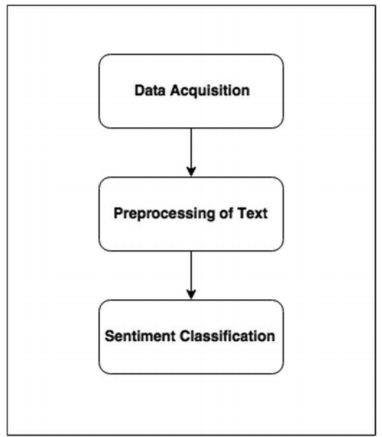
\includegraphics[width=0.6\linewidth]{Screenshot1.png}
\caption{Sentiment Analysis Process}
\end{figure}
\subsubsection{\textbf{Data acquisition}}
Data acquisition is an extremely important phase, since without a well-defined and representative dataset the rest of the process is useless. Today there are several web sites and API that we can use to obtained users’ tweets. In Table 1 we can see some examples of public datasets and their characteristics. For our approach we have constructed the dataset using the Twitter API to obtain the users’ tweets. These tweets are defined in topics such as: Politics, Economics, Tourism and Marketing. \\
\subsubsection{\textbf{Preprocessing of text}}
The preprocessing phase allows to reduce noise in data, reduce its dimension and perform suitable selection of features. There are some techniques that we can use:\\
\begin{itemize}
\item Remove all punctuation, symbols, numbers.
\item Remove stop-words.
\item Remove all URLs (e.g. www.xyz.com), hashtags (e.g. HASHTAG), targets (@username)
\item Stemming: this technique allows to eliminate the endings or beginnings of words and detect their root form.
\item Lowercasing: it is a technique to lower-case all words. By doing so, many words are merged and the dimensionality of document collection is reduced.
\end{itemize}

\subsubsection{\textbf{Sentiment Classification}}
NLP refers to computer systems that process human language in terms of its meaning. NLP understands that several words make a phrase, several phrases make a sentence and, ultimately, sentences convey ideas. NLP works by analyzing language for it's meaning, NLP systems are used for in a number of areas such as converting speech to text, language translation, and grammar checks.Although NLP may seem to be far superior to keyword processing, it still has its limitations. Sarcasm a well known Australian trait, is very difficult to detect using NLP as is hyperbole (exaggerated statements) and social media acronyms (e.g. OMG, BFF, BTW etc) or social jargon such as:\\
\begin{itemize}
\item \textbf{Youturn:} To follow another person on social media with the intention of unfollowing them once they have you followed back, esp. on Twitter
\item \textbf{Wallflower:} A person who regularly consumes the social media of others but never posts
\item \textbf{Face Crawling:} Begging for Facebook likes, online or offline
\item \textbf{Hash-Browning:} The excessive use of hash-tags within a single post
\item \textbf{Meta-pals:} Social media connections that have never personally met\\
\end{itemize}
People express opinions in complex ways for example: the difference between \textbf{"I'm fine!!!"} and \textbf{"I'm fine."}. Also, changing topic mid post can be confusing. There are many uses of the word \textbf{"sick"}.
\begin{enumerate}
\item \textbf{This is so sick. I can’t believe this.}
\item \textbf{The boy is sick!}
\end{enumerate}
Sometimes even human interpretation can be hard to determine. The word sick in the post means \textbf{"cool"} or \textbf{"ill"}?\\
Like this if you think this is \textbf{"sick"}.\\


\begin{figure}[h]
\centering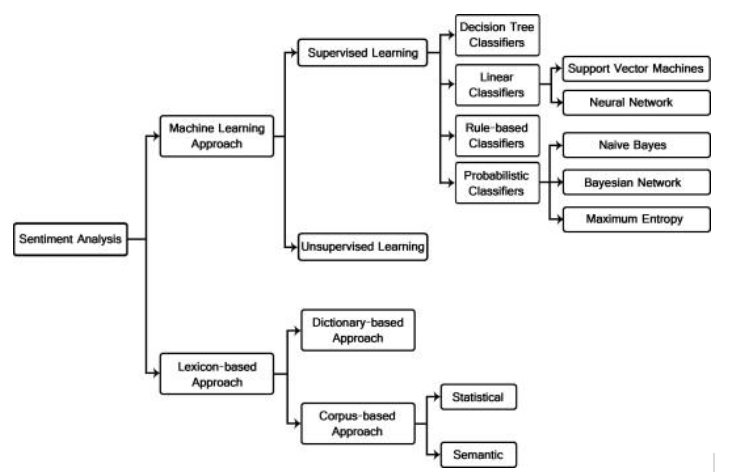
\includegraphics[width=1.2\linewidth]{Screenshot.png}
\caption{Sentiment Analysis Workflow}
\end{figure}

\subsection{\textbf{Machine Learning Approach}}
You’re aware of the basic workings of any Machine Learning algorithms. The same route by followed in ML-based sentiment analysis algorithms as well. These algorithms require you to create a model by training the classifier with a set of example. This ideally means that you must gather a dataset with relevant examples for positive, neutral, and negative classes, extract these features from the examples and then train your algorithm based on these examples. These algorithms are essentially used for computing the polarity of a document.



\subsection{\textbf{Supervised Learning}} 
Supervised learning depends on training documents that contain labels. Usually these labels are obtained by manually labeling by a supervisor, which means that the documents or tweets are cataloged or labeled according to the supervisor previous knowledge and experience. In supervised learning, the training dataset will be used to build the model, and the testing dataset will be used for labeling prediction. Several supervised machine learning techniques have been formulated to classify the tweets into classes, among them we have Support Vector Machine (SVM) and Naive Bayes (NV), which have achieved success in sentiment analysis. \\

%\begin{table}[h]
%\centering
%\begin{tabular}{l l l}
%\hline
%\textbf{Treatments} & \textbf{Response 1} & \textbf{Response 2}\\
%\hline
%Treatment 1 & 0.0003262 & 0.562 \\
%Treatment 2 & 0.0015681 & 0.910 \\
%Treatment 3 & 0.0009271 & 0.296 \\
%\hline
%\end{tabular}
%\caption{Table caption}
%\end{table}



%\begin{figure}[h]
%\centering
\includegraphics[width=0.4\linewidth]{placeholder}
%\caption{Figure caption}
%\end{figure}



%\begin{equation}
%\label{eq:emc}
%e = mc^2
%\end{equation}

\section{RESOURCES REQUIRED}
\label{S:2}

In a Twitter data analytics platform, the visualization must permit data manipulation and filtering in an interactive way, to quickly identify anomalies and outliers.\\
Moreover, it must be able to visualize streaming data at different time resolutions (per years, months, weeks, days, hourly, in real time). Processed data must permit also predictive analytics supporting decision processes, such as regression, predictions, clustering, machine learning. \\
There must be the possibility to extract processed data from the platform, so that they can be processed later independently to identify how they work on analyzing, predicting or early warning of events based on social media data.\\

\begin{itemize}
\item Twitter Metrics: insights about tweets volume metrics (tweets, retweets over time etc.); \\
\item Natural Language Processing (NLP): to extract linguistic information from textual contents, useful for further investigations (e.g., Sentiment Analysis);\\
\item Sentiment Analysis: techniques and solutions adopted to extract a quantitative measure of users’ sentiment from published textual contents; \\
\item API availability: accessibility via API;\\ 
\item Data Sets: Using inbuilt datasets from "tweepy" library defined in Python \\
\item Data analysis based on geolocation (e.g., geographic clustering); \\
\item Real-time analysis: the capability of the system to perform Twitter data analysis on a real-time basis; \\
\item Full faceted search: in order to have further views of data analyzed on tweets collection it is mandatory the exploitation of full faceted search, which enable users to browse tweets by choosing from a predetermined set of categories (tweet author, message, url, geolocation etc.);\\
\end{itemize}

\section{EXPECTED OUTCOME}
\label{S:2}
After the Sentiment Analysis of the Twitter Data through Support Vector Machine (SVM) we'll able to classify the comments, words or phrases among three categories: positive, negative or neutral with more proficiency and higher accuracy.\\
Simply reading a post will let you identify whether the author had a positive stance or a negative stance on the topic – but that’s if you’re well versed in the language. However, a computer has no concept of naturally spoken language – so, we need to break down this problem into mathematics (the language of a computer). It cannot simply deduce whether something contains joy, frustration, anger, or otherwise – without any context of what those words mean.\\
Sentiment Analysis solves this problem by using Natural Language Processing. Basically, it recognizes the necessary keywords and phrases within a document, which eventually help the algorithm to classify the emotional state of the document.\\
Data Scientists and programmers write applications which feeds the documents into the algorithm and stores the results in a way which is useful for clients to use and understand.\\
Keyword spotting is one of the simplest technique and leveraged widely by Sentiment Analysis algorithms. The fed Input document is thoroughly scanned for the obvious positive and negative words like “sad”, “happy”, “disappoint”, “great”, “satisfied”, and such.\\
There are a number of Sentiment Analysis algorithms, and each has different libraries of words and phrases which they score as positive, negative, and neutral. These libraries are often called the “bag of words” by many algorithms.\\
Although this technique looks perfect on the surface, it has some definite shortcomings. Consider the text, “The service was horrible, but the ambiance was awesome!” Now, this sentiment is more complex than a basic algorithm can take into account – it contains both positive and negative emotions. For such cases, more advanced algorithms were devised which break the sentence on encountering the word “but” (or any contrastive conjunction). So, the result becomes “The service was horrible” AND “But the ambiance was awesome.”\\
This sentence will now generate two or more scores (depending on the number of emotions present in the statement). These individual scores are consolidated to find out the overall score of a piece. In practice, this technique is known as Binary Sentiment Analysis.\\
No Machine Learning algorithm can achieve a perfect accuracy of 100percent, and this is no different. Due to the complexity of our natural language, most of the sentiment analysis algorithms are only 80percent accurate, at best.\\


\textbf{References}
\begin{thebibliography}{1}
\bibitem{IEEEhowto:kopka}
Harvesting Opinions in Twitter  for Sentiment Analysis \\
Juan Guevara13, Joana Costa12, Jorge Arroba34, Catarina Silva12 1School of Technology and Management, Polytechnic Institute of Leiria, Portugal 2Center for Informatics and Systems of the University of Coimbra, Portugal 3Universidad Central del Ecuador, Ecuador 4University of Alicante, Spain 2162315@my.ipleiria.pt,{catarina, joana.costa}@ipleiria.pt, jarroba@uce.edu.ec 
\bibitem{}
Sentiment Classification System of Twitter Data for US Airline Service Analysis\\
Ankita Rane Computer Science and Engineering BITS Pilani, Dubai Campus Dubai, UAE ankitarane24@gmail.com
Dr. Anand Kumar Electrical and Electronics Engineering BITS Pilani, Dubai Campus Dubai, UAE akumar@dubai.bits-pilani.ac.in
\bibitem{}
Twitter Vigilance:a Multi-User platform for Cross-Domain Twitter DataAnalytics, NLPand Sentiment Analysis \\
Daniele Cenni, Paolo Nesi, Gianni Pantaleo, Imad Zaza DISIT Lab, Distributed [Systems and internet | Data Intelligence and] Technologies Lab Dep. of Information Engineering (DINFO), University of Florence Florence, Italy,http://www.disit.org,http://www.disit.dinfo.unifi.it paolo.nesi@unifi.it,daniele.cenni@unifi.it
\bibitem{}
Investigating sentiment analysis using machine learning approach\\
Sankar.H
School of Computing,
SASTRA University,
Tanjore, Tamil Nadu, India

Subramaniyaswamy.V
School of Computing,
SASTRA University,
Tanjore, Tamil Nadu, India
\bibitem{}
A Review on: Opinion Mining and Sentiment Analysis based on Natural Language Processing\\
Swati N. Manke, Nitin Shivale JSPM’S BSIOTR Wagholi, Savitribai Phule Pune University
\bibitem{}
Application of Machine Learning Techniques to Sentiment Analysis\\
Anuja P Jain, Asst. Prof Padma Dandannavar
Computer Science and Engineering
Gogte Institute of Technology
Belgaum, India
padmad@git.edu
\bibitem{}
Research on text sentiment analysis based on CNNs and SVM\\
Yuling Chen , Zhi Zhang
Collage of Computer Science and Technology,
Wuhan University of Science and Technology, 2
Hubei Province Key Laboratory of Intelligent Information
Processing and Real-time Industrial System
Wuhan, China, 430065
Email: 1506948905@qq.com
\bibitem{}
A Subword-based Deep Learning Approach for Sentiment Analysis of Political Tweets \\
Marco Pota Institute for High Performance Computing and Networking National Research Council of Italy Naples, Italy marco.pota@icar.cnr.it 
Massimo Esposito Institute for High Performance Computing and Networking National Research Council of Italy Naples, Italy massimo.esposito@icar.cnr.it 
Marco A. Palomino Big Data Group Univeristy of Plymouth Plymouth, UK marco.palomino@plymouth.ac.uk 
Giovanni L. Masala Big Data Group Univeristy of Plymouth Plymouth, UK giovanni.masala@plymouth.ac.uk
 
\end{thebibliography}


%% The Appendices part is started with the command \appendix;
%% appendix sections are then done as normal sections
% \appendix
 %\section{}
 %\label{}

 
%%
%% Following citation commands can be used in the body text:
%% Usage of \cite is as follows:
%%   \cite{key}          ==>>  [#]
%%   \cite[chap. 2]{key} ==>>  [#, chap. 2]
%%   \citet{key}         ==>>  Author [#]

%% References with bibTeX database:

%\bibliographystyle{model1-num-names}
%\bibliography{sample.bib}

%% Authors are advised to submit their bibtex database files. They are
%% requested to list a bibtex style file in the manuscript if they do
%% not want to use model1-num-names.bst.

%% References without bibTeX database:

%\begin{thebibliography}{00}

 %\bibitem must have the following form:
  % \bibitem{key}...
%%

% \bibitem{}

%\end{thebibliography}


\end{document}

%%
%% End of file `elsarticle-template-1-num.tex'.